% 2003 年粤桂卷第 1 题：直线 y = ax 与 y = x + a 选项图
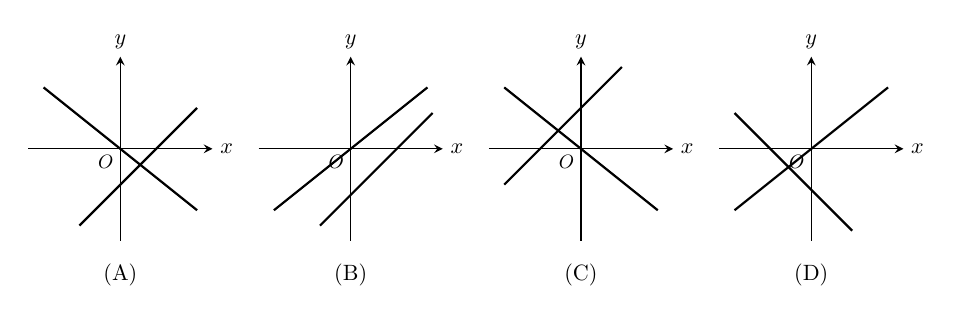
\begin{tikzpicture}[>=stealth,scale=0.65]
  % Subfigure A
  \begin{scope}[shift={(0,0)}]
    \draw[->] (-1.8,0)--(1.8,0) node[right,scale=0.8] {$x$};
    \draw[->] (0,-1.8)--(0,1.8) node[above,scale=0.8] {$y$};
    \node[below left,scale=0.7] at (0,0) {$O$};
    \draw[thick] (-1.5,1.2)--(1.5,-1.2); % y = ax, a < 0
    \draw[thick] (-0.8,-1.5)--(1.5,0.8); % y = x + a, a < 0 (y-intercept < 0, slope = 1)
    \node[below,scale=0.8] at (0,-2.1) {(A)};
  \end{scope}

  % Subfigure B
  \begin{scope}[shift={(4.5,0)}]
    \draw[->] (-1.8,0)--(1.8,0) node[right,scale=0.8] {$x$};
    \draw[->] (0,-1.8)--(0,1.8) node[above,scale=0.8] {$y$};
    \node[below left,scale=0.7] at (0,0) {$O$};
    \draw[thick] (-1.5,-1.2)--(1.5,1.2); % y = ax, a > 0
    \draw[thick] (-0.6,-1.5)--(1.6,0.7); % y = x + a, intercept < 0
    \node[below,scale=0.8] at (0,-2.1) {(B)};
  \end{scope}

  % Subfigure C
  \begin{scope}[shift={(9,0)}]
    \draw[->] (-1.8,0)--(1.8,0) node[right,scale=0.8] {$x$};
    \draw[->] (0,-1.8)--(0,1.8) node[above,scale=0.8] {$y$};
    \node[below left,scale=0.7] at (0,0) {$O$};
    \draw[thick] (-1.5,1.2)--(1.5,-1.2); % y = ax, a < 0
    \draw[thick] (-1.5,-0.7)--(0.8,1.6); % y = x + a, intercept > 0
    \node[below,scale=0.8] at (0,-2.1) {(C)};
  \end{scope}

  % Subfigure D
  \begin{scope}[shift={(13.5,0)}]
    \draw[->] (-1.8,0)--(1.8,0) node[right,scale=0.8] {$x$};
    \draw[->] (0,-1.8)--(0,1.8) node[above,scale=0.8] {$y$};
    \node[below left,scale=0.7] at (0,0) {$O$};
    \draw[thick] (-1.5,-1.2)--(1.5,1.2); % y = ax, a > 0
    \draw[thick] (-1.5,0.7)--(0.8,-1.6); % negative slope
    \node[below,scale=0.8] at (0,-2.1) {(D)};
  \end{scope}
\end{tikzpicture}
